\chapter{Resultados}

{\color{red} Em andamento}

Com o Agente treinado, é possível gerar novas sequências seguindo a arquitetura ilustrada na figura \ref{fig:geradorseq}.
Neste caso, o Agente gerou mais de 200 proteínas diferentes a partir de mutações na sequência inicial. Destas, 63 possuem um TMScore superior a 92\%.

\begin{figure}[H]
    \centering
    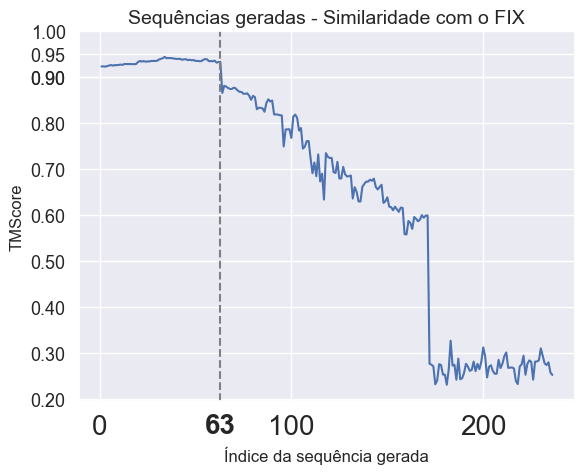
\includegraphics[width=.8\linewidth]{figuras/plot_tmscore_decreasing.png}    
    \caption{Variação da similaridade entre as sequências geradas e o FIX }
    \label{fig:rew_per_ep_train}
  \end{figure}

É interessante notar que, apesar da forte semelhança entre as estruturas, em termos de IS (Idêntidade de Sequência), são proteínas muito diferentes, tendo em média cerca de 30\% de similaridade. 
  
\begin{table}[htbp]
    \centering
    \begin{tabular}{c|cccc}
        \hline
        \textbf{ID} & \textbf{TM-Score} & \textbf{IS - seq. original} \\
        \hline
         20 & 93.33\% & 30.64\% \\
         30 & 93.62\% & 30.21\% \\
         34 & 94.48 & 29.79\% \\
         63 & 93.36 & 26.81\% \\
        \hline
    \end{tabular}
    \caption{Generated proteins}
    \label{tab:tabela_exemplo}
\end{table}

\begin{figure}%
    \centering
    \subfloat[\centering Estrutura Alvo ]{{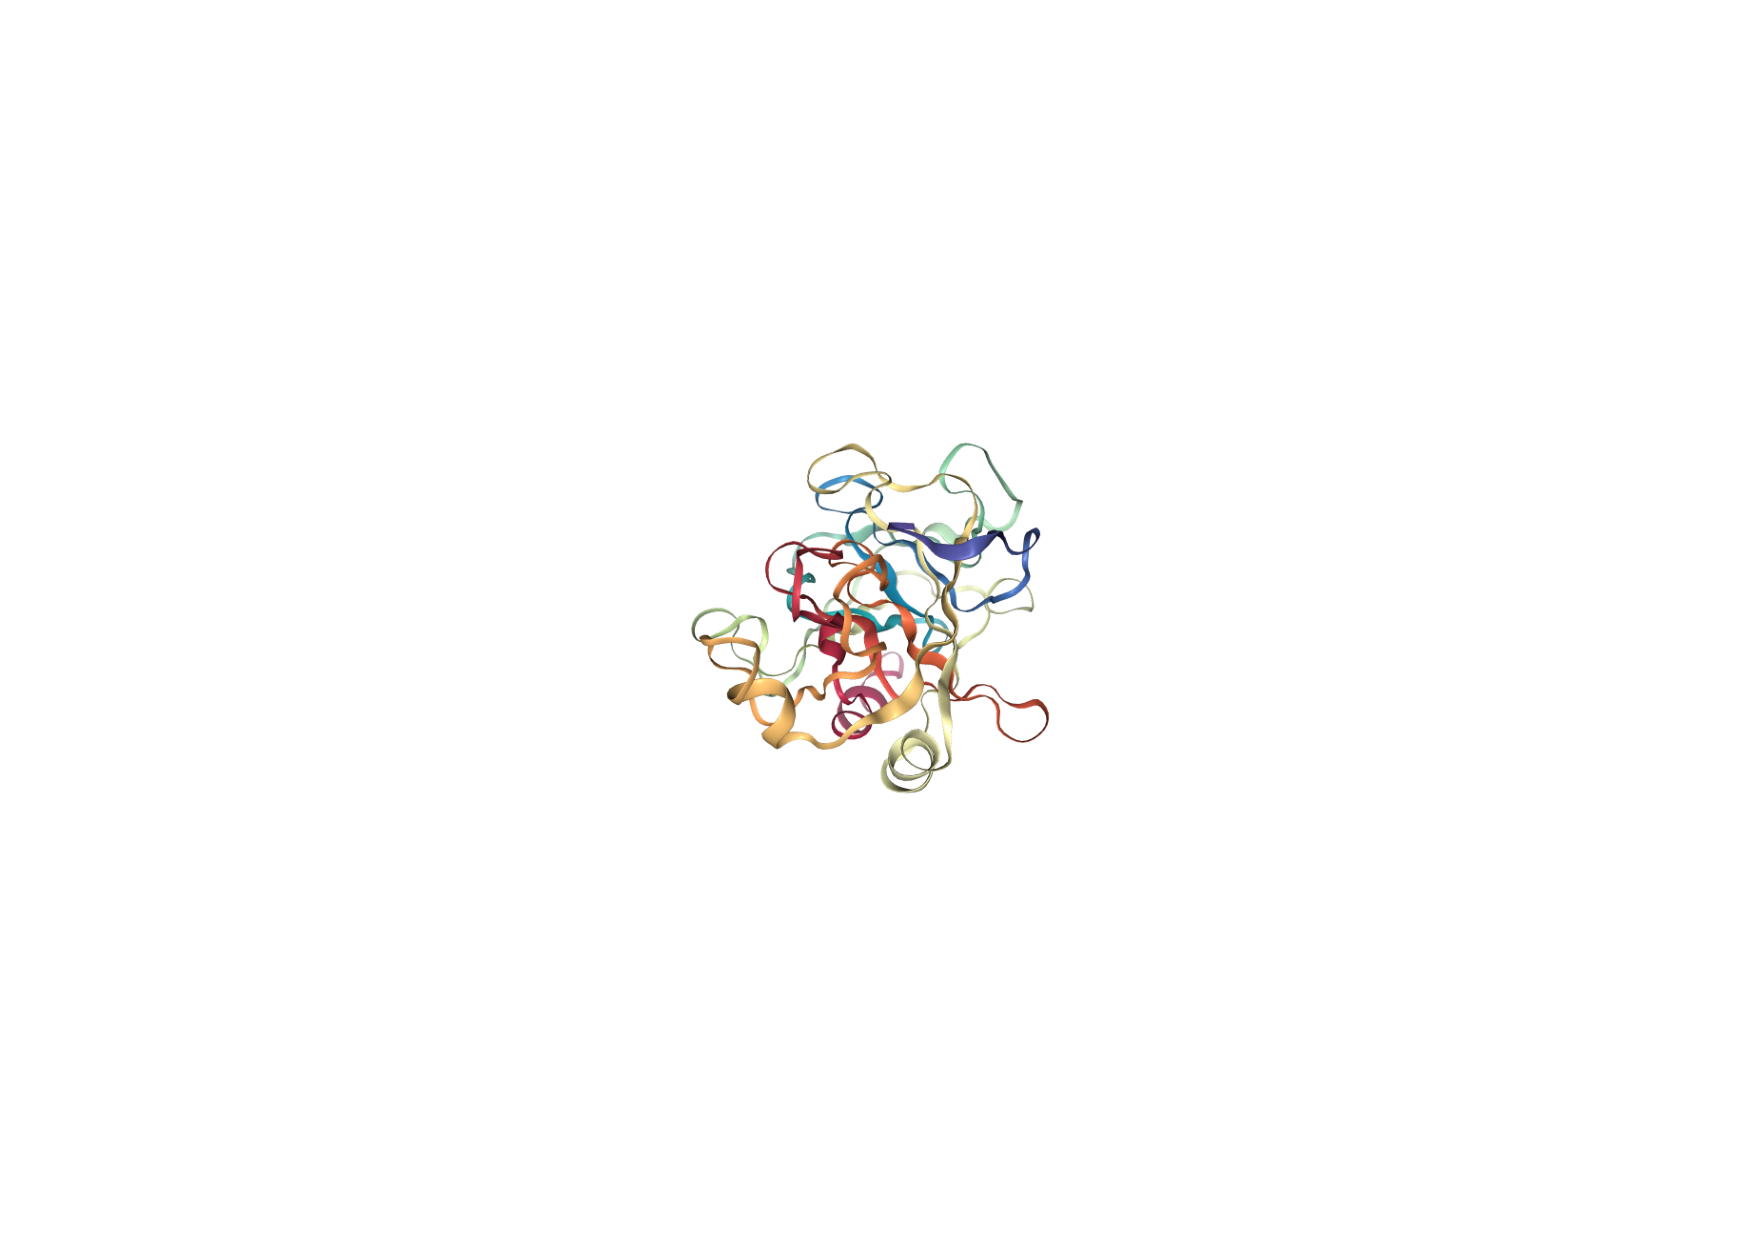
\includegraphics[width=6cm]{figuras/target_structure.pdf} }}%
    \qquad
    \subfloat[\centering Estrutura gerada -  ID 3]{{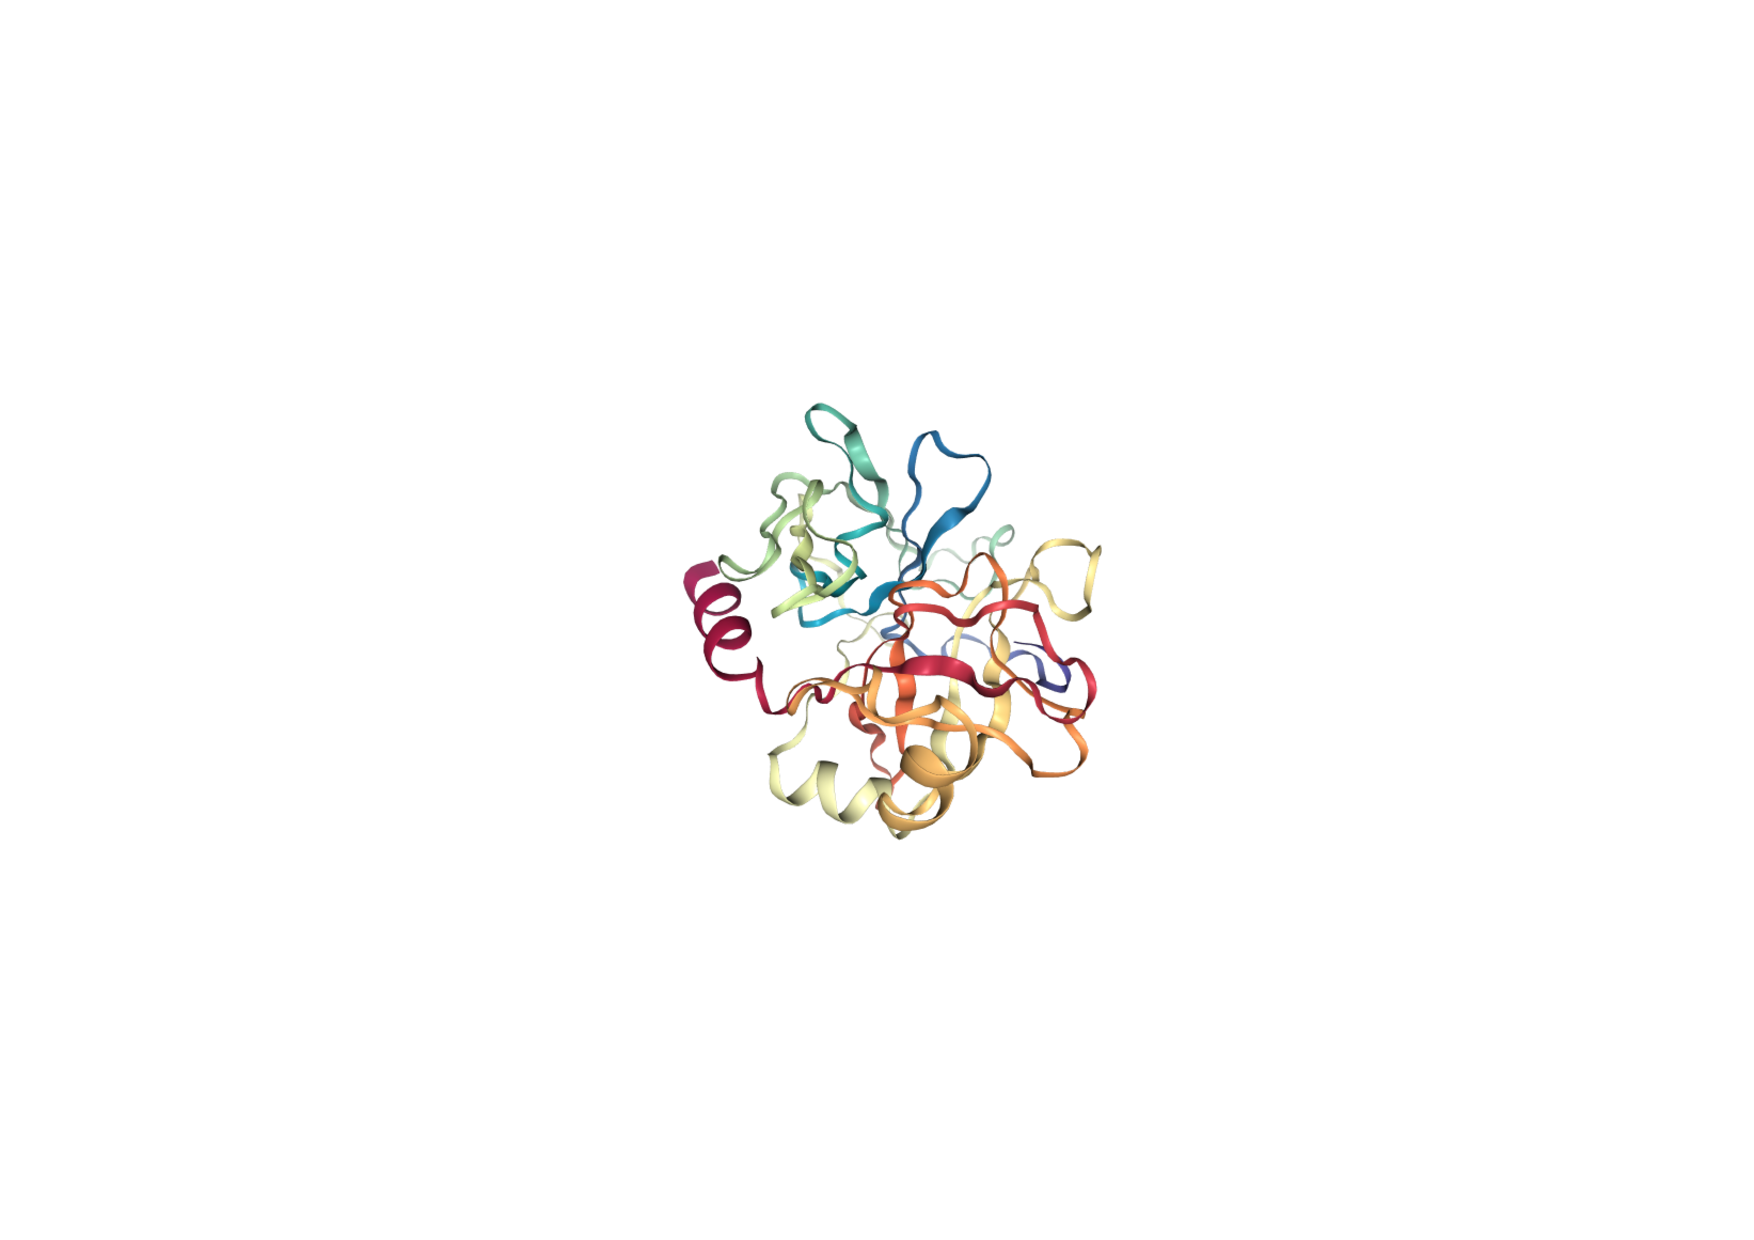
\includegraphics[width=6cm]{figuras/B_v2_tmscore_0.9343_step_41.pdf} }}%
    \caption{Comparação entre estruturas}%
    \label{fig:example}%
\end{figure}

{\color{red} Imagem das proteinas sobrepostas}

{\color{red} Resultados Imuno}

{\color{red} Resultados Docking}